\documentclass{article}
\usepackage[utf8]{vietnam}
%% Math Packages %%%%%%%%%%%%%%%%%%%%%%%%%%%%%%%%%%%%%%%%%%%%
\usepackage{amsmath}
\usepackage{amsthm}
\usepackage{amsfonts}

%%Document package
\usepackage[bookmarks=false,pdfborder={0 0 0}]{hyperref}
\usepackage{listings}
\usepackage{titlesec}
\usepackage{color}
\usepackage{multirow}
\setcounter{secnumdepth}{4}
%% Graphics package
\usepackage{float}
\usepackage{graphicx}
\graphicspath{{images/}}


\input{codestyle.tex}


\newcommand{\tab}[1]{\hspace{.2\textwidth}\rlap{#1}}
\begin{document}

%%Tiêu đề
\thispagestyle{empty}

\begin{titlepage}

\center{\huge{BT01: Phép gán và phép so sánh}}
\center{\Large{Nhập môn phân tích độ phức tạp thuật toán}}

\vfill
\begin{flushright}
\begin{tabular}{l l}
GVLT: &Thầy Trần Đan Thư\\
&\\
GVTH: &Thầy Nguyễn Đức Thân\\
&Thầy Trương Toàn Thịnh\\
&Thầy Nguyễn Vinh Tiệp\\
&Thầy Nguyễn Sơn Hoàng Quốc\\
&\\
Sv: &Nguyễn Phan Mạnh Hùng - 1312727\\
\end{tabular}
\end{flushright}
\end{titlepage}
\pagebreak
\thispagestyle{empty}
\tableofcontents
\pagebreak
%%
\pagenumbering{arabic}
\section{Dãy số Fibonacci}
\subsection{Quy ước}
$C(n)$ là số phép so sánh.\newline
$A(n)$ là số phép gán.\newline
\subsection{Thuật toán đệ quy}
\subsubsection{Mã nguồn}
%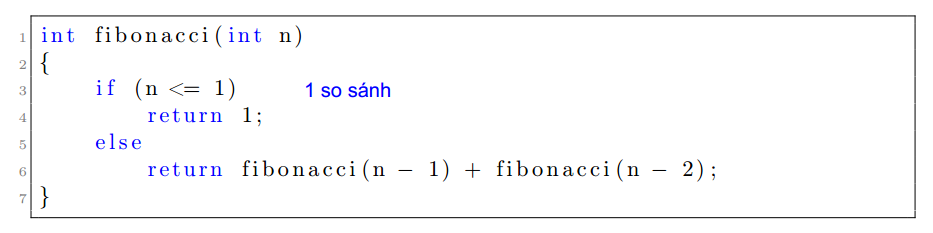
\includegraphics[scale = 0.5]{FiboRecurCounting}
\lstinputlisting[style = C++]{Sources/FibRe.cpp}

\subsubsection{Phép so sánh}
\begin{flushleft}
Ta tính $C(n)$ qua hệ thức truy hồi sau:\\
\begin{equation} \label{eq:Eq1}
C(n) = 
\begin{cases}
	1, & \quad n \in \{ 0, 1 \} \\
	C(n-1) + C(n-2) + 1, & \quad n > 1 
\end{cases} 
\end{equation}

Ta thấy:\\
\begin{center}
	\begin{tabular}{l c c c r}
		$\forall n \geq n_{0} = 2$\\
		$2 \times C(n-2)$ & $\leq$ & $C(n)$ & $\leq$ & $2 \times C(n-1)$\\
		$2 \times C(n-3)$ & $\leq$ & $C(n-1)$ & $\leq$ & $2 \times C(n-2)$\\
		&&\vdots&&\\
		$2 = 2 \times C(0)$ & $\leq$ & $C(2)$ & $\leq$ & $2 \times C(1) = 2$	
	\end{tabular}
\end{center}

nên $2^{\frac{n}{2}}   < C(n) <  2^{n-1} < 2^n \forall n \geq n_{0} = 2 $\\
do đó
\begin{gather}
	C(n) \in O(2^{n})
	C(n) \in \Omega (2^{\frac{n}{2}})
\end{gather}

%Mà:
%\begin{gather}
% \lim_{n\to\infty} 2^{\frac{n}{2}} = \lim_{n\to\infty}(2*\frac{1}{\sqrt{(2)}})^n 
%\end{gather}


Giải hệ thức (\ref{eq:Eq1}), ta được:\\
\begin{equation}\label{eq:Eq3}
C(n) = \frac{2}{\sqrt{5}}  \times \left( \left( \frac{1+\sqrt{5}}{2} \right) ^{n+1} - \left( \frac{1-\sqrt{5}}{2} \right) ^{n+1} \right)-1
\end{equation}
Dựa vào công thức trên, ta có thể chặn trên sát hơn như sau:
\begin{gather}
\begin{align*}
	\forall n \geq n_{0} = 2, M = 5\\
 	C(n)  &\leq \frac{2}{\sqrt{5}}  \times \left( \left|  \frac{1+\sqrt{5}}{2} \right| ^{n+1} + \left| -\frac{1-\sqrt{5}}{2} \right| ^{n+1} \right)\\
	&\leq \frac{2}{\sqrt{5}}  \times 2 \times  \left|  \frac{1+\sqrt{5}}{2} \right| \times  \left|  \frac{1+\sqrt{5}}{2} \right| ^{n} \\
	&\leq M \times \left|  \frac{1+\sqrt{5}}{2} \right| ^{n}\\
	\Rightarrow &~~ C(n) \in O \left( \left( \frac{1+\sqrt{5}}{2} \right) ^{n}  \right)
\end{align*}
\end{gather}

Bên cạnh đó, dựa vào \ref{eq:Eq3}
\begin{gather}
	C(n) \in \Theta \left( \frac{2}{\sqrt{5}}  \times \left( \left( \frac{1+\sqrt{5}}{2} \right) ^{n+1} - \left( \frac{1-\sqrt{5}}{2} \right) ^{n+1} \right)-1 \right) 
\end{gather}
\end{flushleft}

\subsubsection{Phép gán}
\begin{flushleft}
Ta thấy trong cách cài đặt bằng đệ quy thì không có phép gán nào nên ta xem như:
\begin{equation}
A(n) = 0
\end{equation}
Nếu ta xem \emph{return} cũng như 1 phép gán thì ta thấy $A(n) = C(n)$.
\end{flushleft}
\subsection{Thuật toán không đệ quy}
\subsubsection{Mã nguồn}
%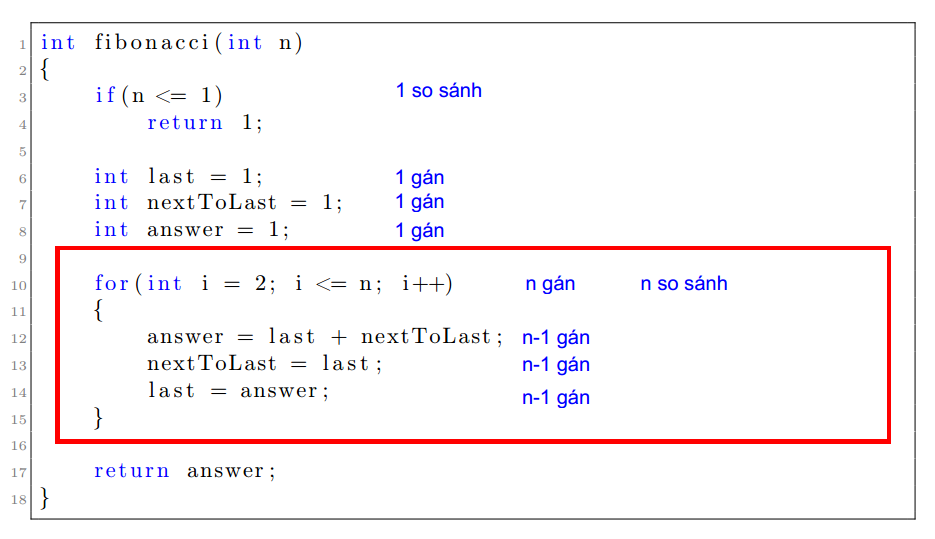
\includegraphics[scale = 0.5]{FiboLoopCounting}
\lstinputlisting[style = C++]{Sources/FibLo.cpp}
\subsubsection{Phép so sánh}
\begin{equation}
C(n) = 
\begin{cases}
1 & \quad n \leq 1\\
n+1 & \quad n > 1\\
\end{cases}
\end{equation}
\subsubsection{Phép gán}
\begin{equation}
A(n) =  3 + n + 3 \times (n-1) = 4*n
\end{equation}
Vậy: 
\begin{equation}
	A(n) \in O(n)
\end{equation}
Do: $\forall n \geq n_{0} = 1$ và $M = 5$ thì $|A(n)| \leq M \times |n|$.\\
Chứng minh tương tự, ta có
\begin{equation}
	A(n) \in \Omega (n)
\end{equation}
do đó:
\begin{equation}
	A(n) \in \Theta (n)
\end{equation}
\subsection{Kết quả thực nghiệm}
\subsubsection{Thuật toán đệ quy}
\begin{tabular}{c|c c c}
	Input & \multicolumn{2}{c}{Output}\\
	&Fib(n) & So sánh & Gán\\
	\hline
	0 & 1 & 1 & 0\\
	1 & 1 & 1 & 0\\
	2 & 2 & 3 & 0\\
	3 & 3 & 5 & 0\\
	4 & 5 & 9 & 0\\
	5 & 8 & 15 & 0\\
	6 & 13 & 25 & 0\\
	7 & 21 & 41 & 0\\
	8 & 34 & 67 & 0\\
	9 & 55 & 109 & 0\\
	10 & 89 & 177 & 0\\
	11 & 144 & 287 & 0\\
	12 & 233 & 465 & 0\\
	13 & 377 & 753 & 0\\
	14 & 610 & 1219 & 0\\
\end{tabular}


\subsubsection{Thuật toán không đệ quy}
\begin{tabular}{c|c c c}
	Input & \multicolumn{2}{c}{Output}\\
	Fib(n) & So sánh & Gán\\
	\hline
	0 & 1 & 1 & 0\\
	1 & 1 & 1 & 0\\
	2 & 2 & 3 & 8\\
	3 & 3 & 4 & 12\\
	4 & 5 & 5 & 16\\
	5 & 8 & 6 & 20\\
	6 & 13 & 7 & 24\\
	7 & 21 & 8 & 28\\
	8 & 34 & 9 & 32\\
	9 & 55 & 10 & 36\\
	10 & 89 & 11 & 40\\
	11 & 144 & 12 & 44\\
	12 & 233 & 13 & 48\\
	13 & 377 & 14 & 52\\
	14 & 610 & 15 & 56\\
\end{tabular}

\subsection{Đồ thị - Nhận xét}
\begin{figure}[H]
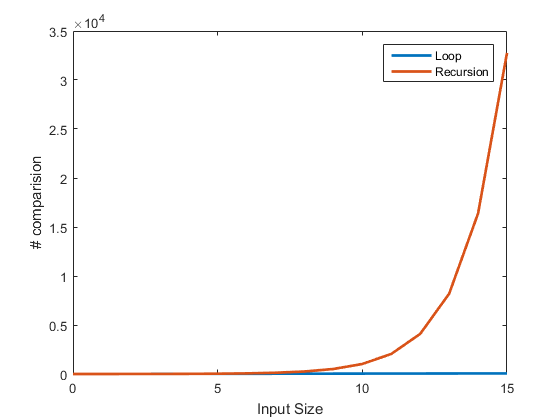
\includegraphics[scale = 1]{Graph}
\caption{Đồ thị biểu diễn số lượng phép so sánh theo n của thuật toán tính số Fibonacci thứ n bằng đệ quy và vòng lặp} 
\end{figure}
\begin{flushleft}
Ta nhận thấy, số phép so sánh (tương tự với phép gán) trong cách cài đặt đệ quy lớn hơn rất nhiều so với cách cài đặt không đệ quy. Điều này khá dễ hiểu do số phép so sánh trong cài đặt đệ quy tăng theo hàm mũ, còn trong cài đặt vòng lặp thì tuyến tính với n.
\end{flushleft}        
\end{document}